
\section{Software Architecture}
\label{sec:software_arch}

This software backbone supports the perception modules presented in Section~\ref{sec:perception_sensing}.

% REORG_TAG: moved here from ROS2 Architecture Design and Implementation
\subsection{ROS2 System Design}

The legacy monolithic Python architecture running on Raspberry Pi created critical limitations for real-time robotics applications: unreliable inter-process communication, insufficient computational parallelization, and poor scalability for advanced perception tasks. These constraints prevented effective utilization of modern multi-core processors and hindered integration of computationally intensive algorithms such as SLAM and human pose detection.

The migration to ROS2 framework addresses these fundamental limitations through its Data Distribution Service (DDS) middleware, which provides robust inter-process communication with Quality of Service guarantees for reliable data transmission under high computational loads. The distributed architecture enables optimal utilization of the NVIDIA Orin Nano's multi-core ARM Cortex-A78AE CPU and integrated GPU, allowing critical processes like SLAM computation, human pose detection, and sensor fusion to execute in parallel without blocking the main control loop. The standardized message interfaces and automatic discovery mechanisms facilitate seamless integration of new sensors while ensuring deterministic message delivery for time-critical operations.

This architectural foundation enables sophisticated multi-node processing capabilities that support real-time VR interaction, advanced perception algorithms, and reliable hardware control—capabilities that form the basis for the specialized node structure detailed in the following subsection.

\subsubsection{Tino's Physical Architecture}

Before examining the software node structure, it is essential to understand Tino's physical composition to provide context for the control systems described throughout this section. Tino is a mobile social robot designed with a distinctive non-anthropomorphic form that prioritizes expressive movement over human-like appearance.

The robot consists of four main physical components: a mobile \textbf{base} that provides differential drive locomotion using two powered wheels and a rear caster wheel (Figure~\ref{fig:tino_on_new_base}); a cylindrical \textbf{body} that houses the computational hardware (NVIDIA Orin Nano), power systems, and internal electronics while maintaining Tino's characteristic fabric-covered aesthetic; an articulated \textbf{head} mechanism that utilizes a three-degree-of-freedom Stewart platform configuration with servo motors to provide expressive pan, tilt, and pitch movements essential for social interaction (Figure~\ref{fig:head_arm_v2}); and a single-actuator \textbf{leg} mechanism that extends from the body to enable coordinated gestures synchronized with base movement.

\begin{figure}[H]
    \centering
    \begin{minipage}{0.3\textwidth}
        \centering
        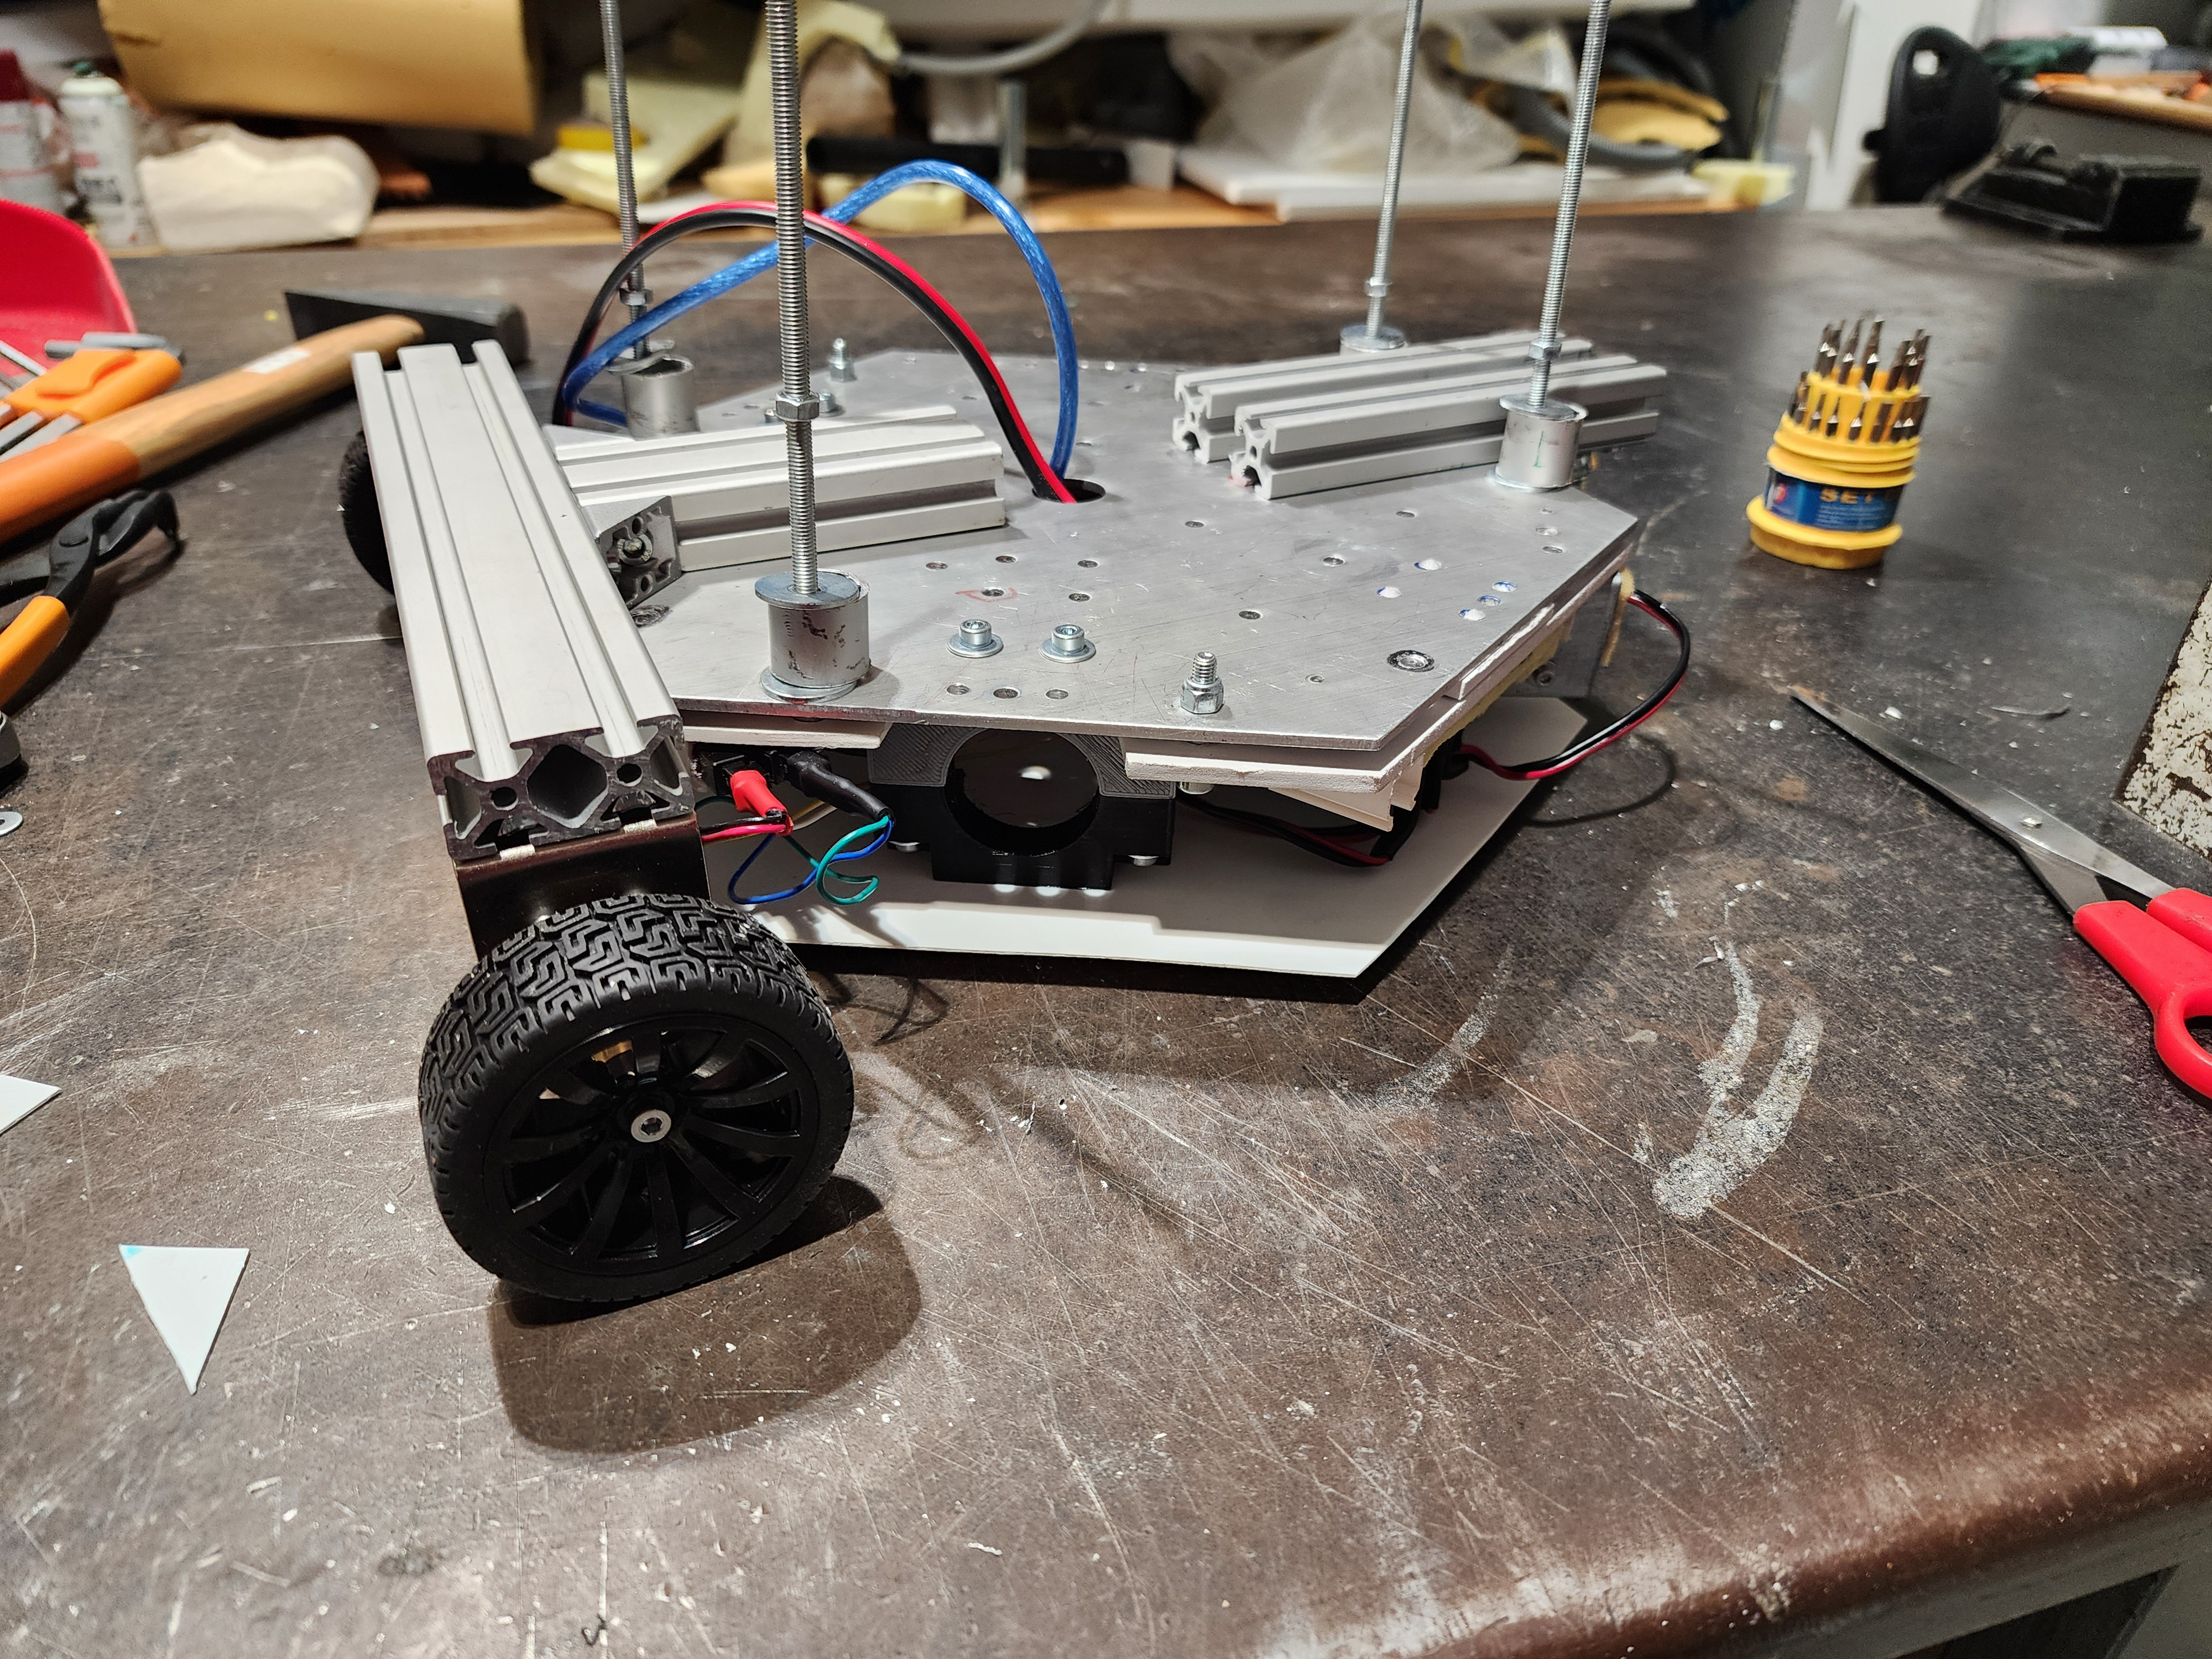
\includegraphics[width=\textwidth]{Images/NewBaseDifferentialDrive.jpg}
        \caption{Differential Drive Base System}
        \label{fig:base_component}
    \end{minipage}
    \quad
    \begin{minipage}{0.3\textwidth}
        \centering
        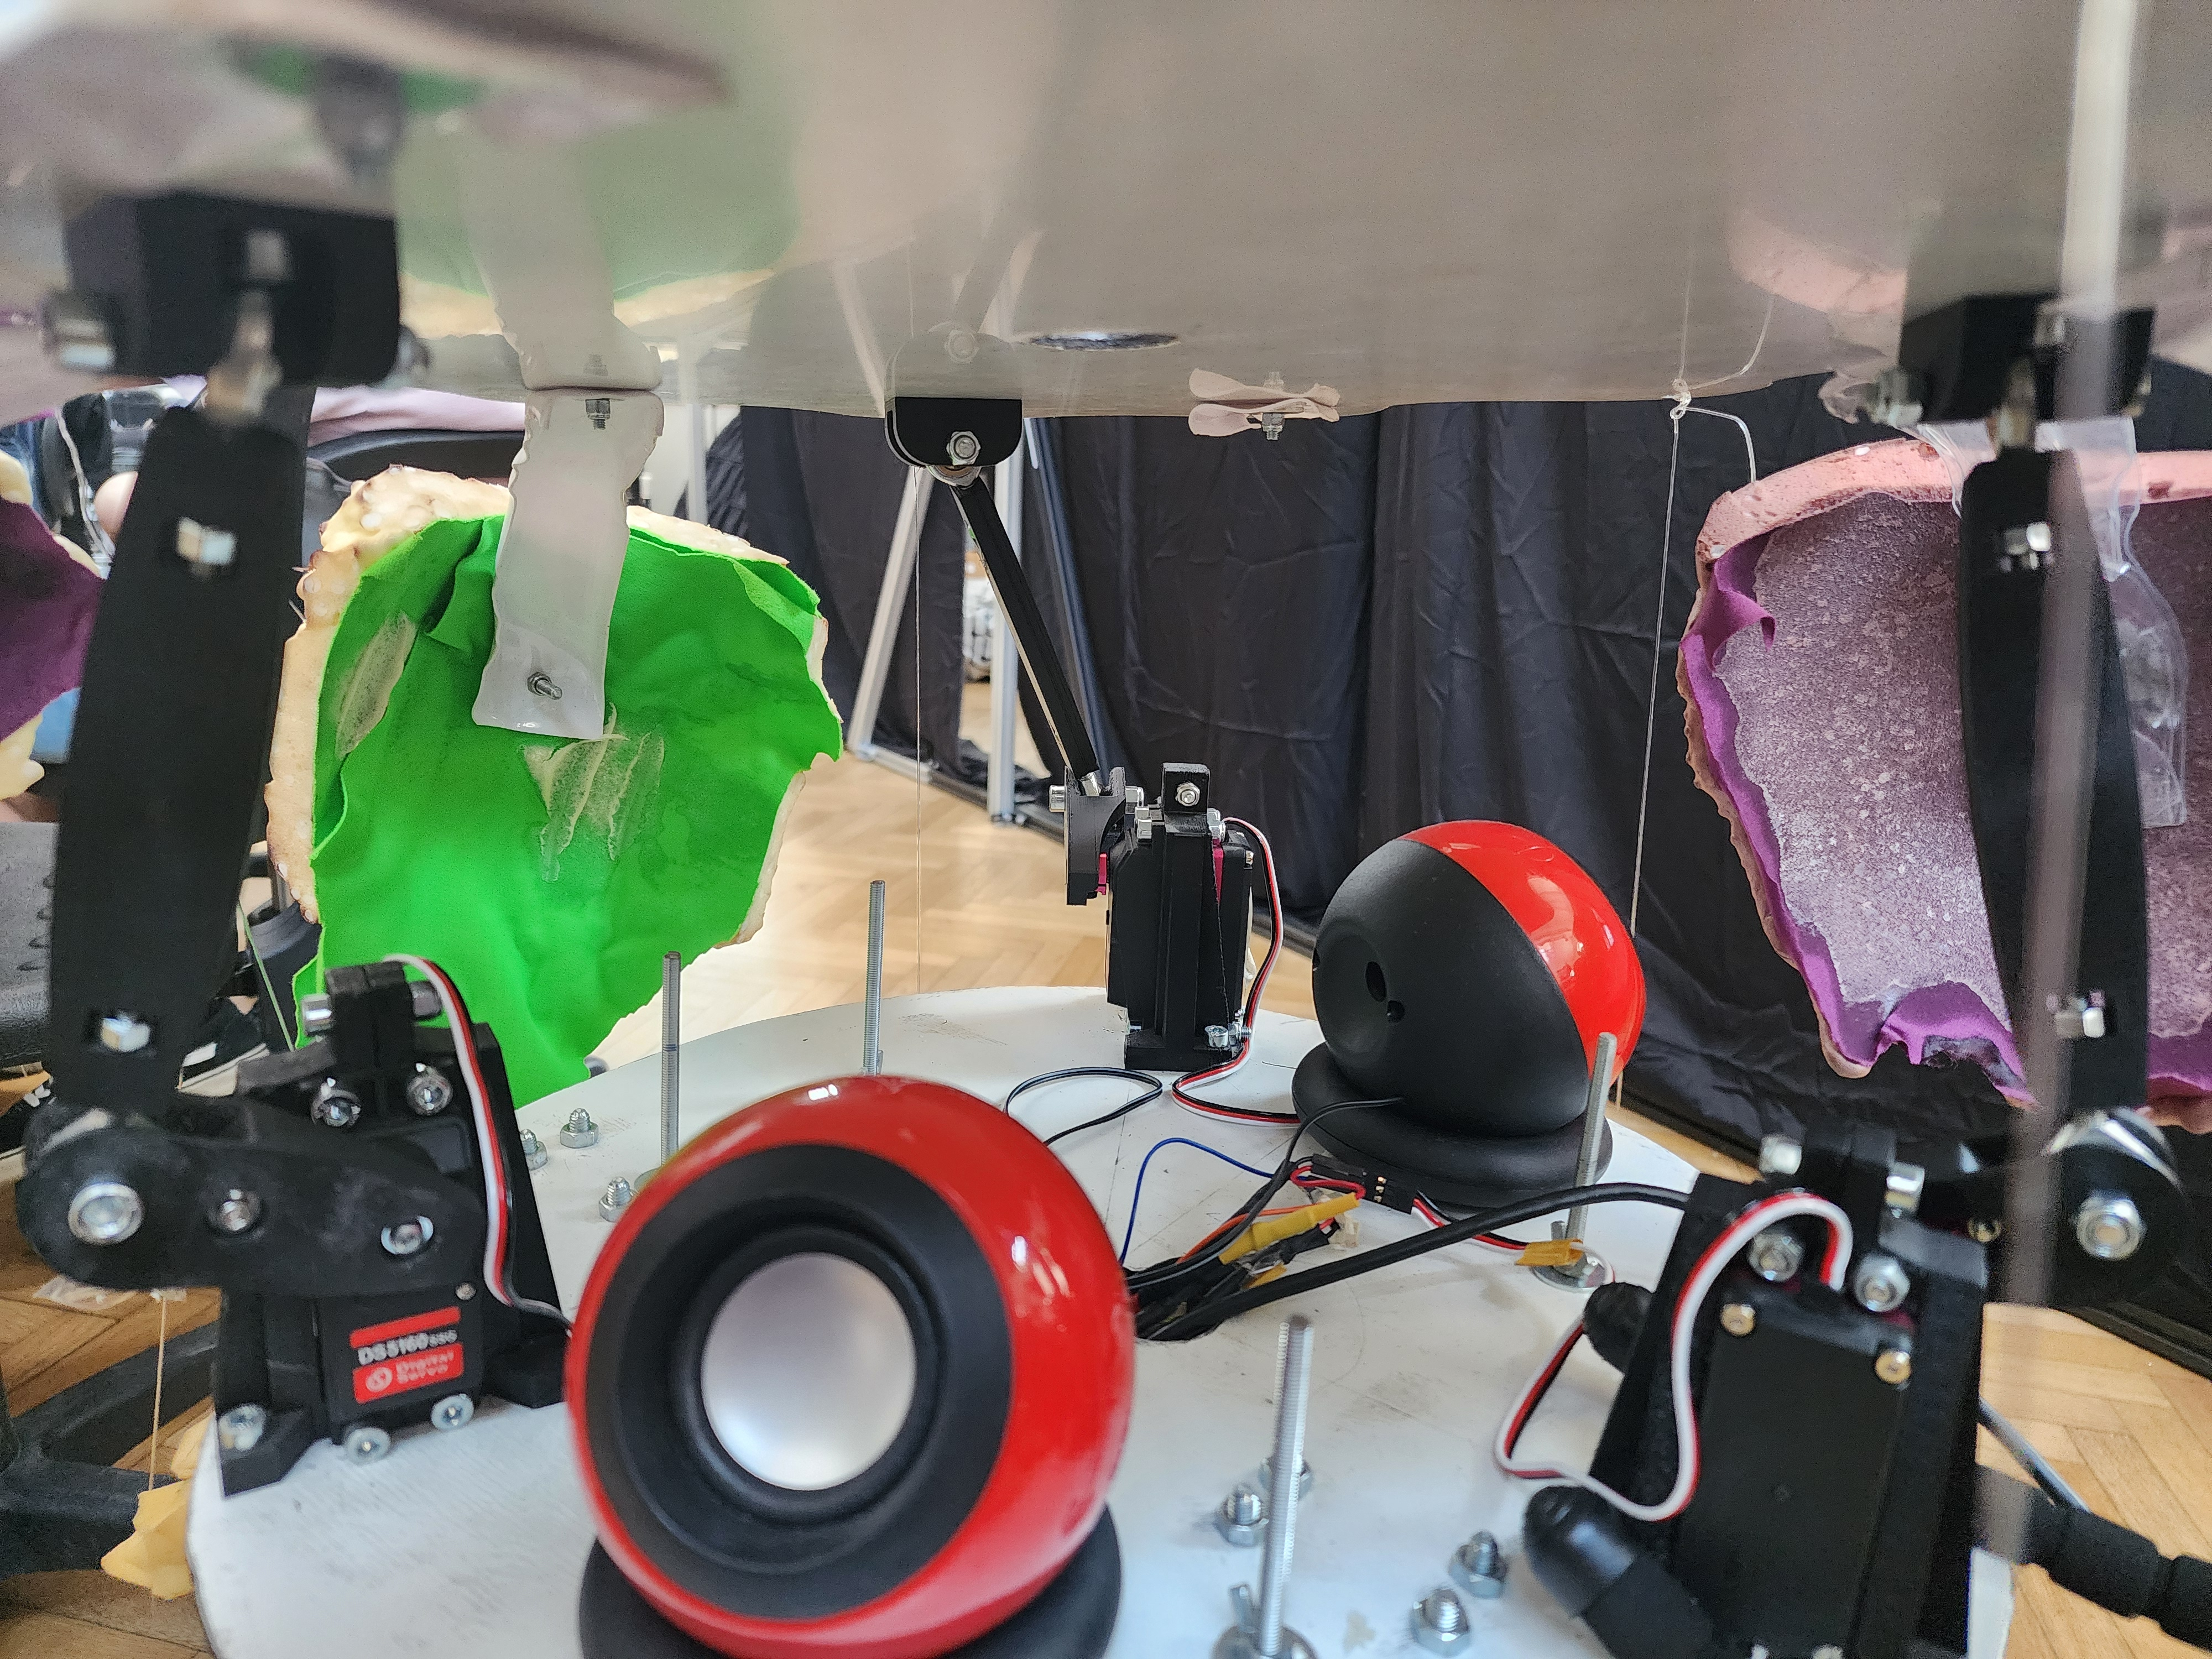
\includegraphics[width=\textwidth]{Images/NewHeadDoubleJoint (2).jpg}
        \caption{Stewart Platform Head Mechanism}
        \label{fig:head_component}
    \end{minipage}
    \quad
    \begin{minipage}{0.3\textwidth}
        \centering
        \includegraphics[width=\textwidth]{Images/leg_detail.jpg}
        \caption{Single-Actuator Leg Mechanism}
        \label{fig:leg_component}
    \end{minipage}
\end{figure}

This modular architecture enables each component to be controlled independently through dedicated Arduino microcontrollers while supporting coordinated behaviors essential for natural social interaction. The head platform provides fine-grained articulation for attention direction and social signaling, while the differential drive base ensures reliable mobility across various indoor environments. The leg mechanism enables expressive gestures that can be precisely coordinated with base movement to create natural locomotion patterns.

The complete robot assembly measures approximately 1.2 meters in height with the fabric head covering, creating an approachable scale for human interaction while housing sophisticated perception hardware including stereo cameras for SLAM and human detection capabilities. Figure~\ref{fig:tino_before_upgrade} and Figure~\ref{fig:tino_after_upgrade} in Section~\ref{sec:hardware_impl} illustrate Tino's external appearance before and after the V2 hardware upgrades, demonstrating how the enhanced internal capabilities were implemented while preserving the robot's distinctive social interaction aesthetic.

\subsubsection{Node Structure and Functionality}

Complex robotics systems require specialized subsystem management to handle diverse hardware interfaces, real-time perception processing, and external system integration without creating bottlenecks or single points of failure. The Tino V2 architecture addresses this through six specialized ROS2 nodes, each responsible for specific functionality while maintaining loose coupling through standardized message interfaces. The perception-focused nodes (Robot Controller for SLAM integration and Pose Detection for human tracking) are described here in terms of their architectural role, with detailed implementation specifics covered in Section~\ref{sec:perception_sensing}.

\paragraph{Gamepad Control Node}

Development and testing of robotic systems requires reliable manual control interfaces that can replicate VR command patterns for validation purposes. The \texttt{gamepad\_node.py} addresses D-input to X-input compatibility issues on Linux while implementing pulse generation mechanisms that replace continuous joystick input with discrete 3-cycle command pulses (120ms duration at 25Hz). Button mapping follows VR command structure: face buttons control leg states (X=1, Y=2, B=3, A=0) and bumpers trigger rotation commands. This node enables comprehensive testing of robot behaviors without VR hardware dependency, ensuring system reliability during development phases. A more detailed analysis of the underlying control architecture and the complete pulse-based command system that enables this seamless VR-gamepad compatibility will be examined in Section~\ref{sec:control_implementation}.

\begin{figure}[H]
    \centering
    \includegraphics[width=0.8\textwidth]{Images/gamepadnode.png}
    \caption{RQT Graph visualization of the Gamepad Control Node showing topic connections and data flow patterns.}
    \label{fig:rqt_gamepad_node}
\end{figure}

\paragraph{Hardware Interface Node}

Multiple Arduino subsystems with individual serial interfaces create device identification and communication coordination challenges that require robust connection management. The \texttt{hardware\_interface\_node.py} manages parallel serial communication with three Arduino subsystems through persistent device symlinks (\texttt{/dev/ttyBASE}, \texttt{/dev/ttyLEG}, \texttt{/dev/ttyHEAD}) created via udev rules. Each thread operates at 115200 baud with configurable message repetition and command format \texttt{BF:value\_BB:value\_HP:value\_HX:value\_HY:value}. Automatic device discovery, connection monitoring, and graceful degradation enable reliable hardware control even when individual subsystems become unavailable, providing the foundation for coordinated movement execution.

\begin{figure}[H]
    \centering
    \includegraphics[width=0.8\textwidth]{Images/hardwarenode.png}
    \caption{RQT Graph visualization of the Hardware Interface Node showing topic subscriptions and Arduino communication patterns.}
    \label{fig:rqt_hardware_interface_node}
\end{figure}

\paragraph{Robot Controller Node}

Advanced robotics systems require centralized coordination to manage sensor fusion, localization monitoring, and behavior orchestration while preventing conflicts between subsystems. The \texttt{robot\_controller\_node.py} implements sophisticated localization supervision including RTAB-Map orientation loss detection (quaternion: x=1.0, y=0.0, z=0.0, w=0.0), automatic odometry reset via \texttt{/reset\_odom} service, and orientation estimation from movement history when RTAB-Map becomes unreliable. Sensor fusion combines UWB absolute positioning with RTAB-Map orientation data, applying 11.5-degree rotation correction to align coordinate frames, then publishes unified pose data to \texttt{/vr\_in/robot\_pose}. This central coordination enables reliable localization and seamless communication with VR systems while providing comprehensive system health monitoring.

\begin{figure}[H]
    \centering
    \includegraphics[width=0.8\textwidth]{Images/robotcontrollernode.png}
    \caption{RQT Graph visualization of the Robot Controller Node showing sensor fusion topic connections and VR pose data publication.}
    \label{fig:rqt_robot_controller_node}
\end{figure}

\paragraph{Pose Detection Node}

Real-time human interaction requires robust detection and tracking capabilities that can provide accurate 3D positioning for VR integration and social robotics research. The \texttt{pose\_detection\_node.py} implements YOLOv11 optimized with TensorRT for Orin Nano performance, combining 2D pose estimation with stereo depth information from Oak-D Pro cameras (\texttt{/right/image\_rect}, \texttt{/stereo/depth}). The system publishes detection results to multiple topics: human position data \linebreak(\texttt{/human\_position}), visualization markers (\texttt{/human\_skeleton}), and structured pose arrays (\texttt{/human\_skeleton\_poses}) with exactly 17 COCO-format joints. Closest-person selection algorithms and temporal smoothing ensure consistent 3D positioning across varying distances, enabling precise human tracking for VR interaction scenarios.

\begin{figure}[H]
    \centering
    \includegraphics[width=0.8\textwidth]{Images/posenode.png}
    \caption{RQT Graph visualization of the Pose Detection Node showing stereo camera topic subscriptions and human tracking data publication.}
    \label{fig:rqt_pose_detection_node}
\end{figure}

\paragraph{VR Integration Node}

VR system integration requires comprehensive bidirectional communication between Unity VR environments and robot systems, addressing challenges in real-time responsiveness, spatial coordination, and user experience consistency while supporting audio feedback capabilities. The \texttt{vr\_interface\_node.py} implements a sophisticated multi-threaded architecture that consolidates all VR communication through custom UDP protocols optimized for ultra-low latency and deterministic message delivery.

The three-port UDP architecture isolates data streams to prevent interference: port 5005 handles incoming 32-byte VR command packets at expected 25Hz rate, port 5006 transmits 24-byte robot pose data at 10Hz, and port 5007 streams 208-byte skeleton data at 10Hz. This isolation enables independent optimization for different latency requirements while supporting flexible deployment through configurable IP addresses (default 192.168.0.201). Traditional ROS2 bridge solutions introduce excessive overhead for real-time VR scenarios, necessitating this custom protocol optimized for robot-VR interaction patterns.

Incoming VR commands utilize binary format with \texttt{struct.unpack('fffiiffi', data)} containing head control floats (pitch/pan/tilt), base command integers (state 0--3, angular direction --1/0/1), and audio parameters (volume 0--255, orientation --1.0 to 1.0) with message ordering validation. The node processes these commands through dedicated listener threads with 1-second timeouts and publishes corresponding movement commands to \texttt{/vr\_out/cmd\_vel} and \texttt{/vr\_out/head\_cmd} topics.

Outgoing data transmission provides continuous robot state information through 24-byte pose packets (position coordinates, orientation quaternion, audio volume) and 208-byte skeleton data containing exactly 17 COCO-format joints with default (0,0,0) coordinates for missing joints. Audio integration enables bidirectional communication where the node receives audio output from \texttt{/vr\_in/audio\_output} topics and processes VR audio control parameters including volume control (0--255) and spatial orientation (--1.0 to 1.0) for real-time audio modification based on VR user interaction and spatial positioning.

The audio control system utilizes ROS2 topics to enable dynamic audio modification based on VR user interaction and robot state. Volume control implementation applies logarithmic scaling to provide natural perceived loudness variations, while orientation-based parameter modulation enables frequency shifting and audio characteristic changes based on spatial positioning, creating spatial audio awareness that enhances immersive VR interaction. The stereo speaker system provides sophisticated spatial audio through quadratic intensity scaling with exponential panning response, creating pronounced left-right separation that follows VR user head movements without audible artifacts.

Communication health monitoring implements comprehensive reliability features including message rate validation against configured targets, connection status tracking with 3-second disconnection timeout, message ordering validation for duplicate/loss detection, and automatic recovery with counter reset upon reconnection. This robust foundation enables immersive robot control through natural VR gestures while providing comprehensive environmental awareness and responsive audio feedback that enhances social presence and interaction naturalness.

\begin{figure}[H]
    \centering
    \includegraphics[width=0.8\textwidth]{Images/vrnode.png}
    \caption{RQT Graph visualization of the VR Interface Node showing bidirectional topic connections for VR communication and data exchange.}
    \label{fig:rqt_vr_interface_node}
\end{figure}

\subsubsection{Communication Protocols and Message Design}

Distributed robotics systems require reliable message exchange mechanisms that can handle diverse data types, latency requirements, and failure scenarios without compromising system performance. The ROS2 communication infrastructure implements a topic-based publish-subscribe architecture with Quality of Service policies optimized for robot pose data (reliable delivery, history depth 10), real-time human tracking (best-effort for continuous streams), and critical movement commands (reliable delivery with immediate processing).

The message hierarchy follows logical data flow patterns: VR input topics \linebreak(\texttt{/vr\_out/cmd\_vel}, \texttt{/vr\_out/head\_cmd}) carry external commands, internal processing topics (\texttt{base\_cmd\_vel}, \texttt{head\_cmd}) handle robot control, and output topics \linebreak(\texttt{/vr\_in/robot\_pose}, \texttt{/vr\_in/human\_position}) provide data to external systems. Robot pose utilizes \texttt{geometry\_msgs/PoseStamped} with high-precision timestamps for sensor fusion, while human detection employs \texttt{geometry\_msgs/PoseArray} containing exactly 17 COCO-format joints with consistent 3D coordinates. VR commands leverage \linebreak\texttt{geometry\_msgs/Twist} where \texttt{linear.x} carries leg states (0--3) and \texttt{angular.z} carries rotation commands (--1, 0, 1).

Synchronous operations utilize ROS2 service calls, particularly the \texttt{/reset\_odom} service (\texttt{std\_srvs/Empty}) for RTAB-Map odometry reset when orientation loss is detected. This communication foundation provides the infrastructure necessary for sophisticated audio generation systems that enhance robot personality and social interaction capabilities, as detailed in the following subsection.

\begin{figure}[H]
    \centering
    \includegraphics[width=\textwidth]{Images/fulltinonodes.png}
    \caption{Complete RQT Graph visualization showing all Tino V2 ROS2 nodes operating simultaneously, illustrating the comprehensive communication architecture with all topic connections, service calls, and data flow patterns across the entire robotic system.}
    \label{fig:rqt_complete_system}
\end{figure}

\begin{figure}[H]
    \centering
    \includegraphics[width=\textwidth]{Images/TinoWithRTAB.png}
    \caption{Comprehensive RQT Graph visualization including RTAB-Map SLAM system and stereo camera nodes alongside all Tino V2 custom nodes. Note: Due to the extensive number of nodes and interconnections in the complete perception pipeline, this visualization may appear complex and dense, but demonstrates the full operational scope of the integrated robotic system.}
    \label{fig:rqt_complete_system_with_rtab}
\end{figure}

\subsection{Dynamic Audio Generation}

Social robotics research requires expressive audio capabilities that enhance robot personality and enable emotional communication beyond visual cues. Traditional robotic audio systems use pre-recorded sounds or basic text-to-speech, limiting the range of emotional expression and adaptability to real-time interaction contexts. Tino's character demands an audio personality that conveys mystery and presence while supporting dynamic modification through external control systems.

The dynamic audio generation system creates custom ambient audio inspired by the No-Face character from Studio Ghibli films, implementing sophisticated breathing simulation algorithms that create natural, organic audio expression. The breathing simulation utilizes a state machine with inhale and exhale phases, implementing sinusoidal wave patterns with randomized duration (2.5--4.0 seconds) and volume variations (0.55--0.75 amplitude) to create natural breathing rhythm variations that avoid monotonous repetition.

Multi-tone synthesis combines three carefully selected base frequencies (110Hz, 146.83Hz, 73.42Hz) with pre-calculated gain values to create rich harmonic content that provides depth and character to the audio output. The frequency selection creates subtle beating patterns and harmonic interactions that enhance the mysterious quality essential to Tino's character expression. Filtered breath noise generation utilizes a first-order low-pass filter applied to random noise, creating organic texture that varies dynamically with breathing intensity and provides natural variation in the audio signature.

The audio system architecture supports real-time parameter modification through ROS2 topic interfaces, enabling external systems to influence audio characteristics including volume scaling, frequency modulation, and spatial positioning. This flexible architecture allows integration with various control systems while maintaining the core audio generation algorithms that define Tino's distinctive audio personality, supporting both autonomous operation and interactive control scenarios essential for social robotics research applications.

The comprehensive software architecture detailed throughout this section provides the foundational framework that enables Tino V2's advanced perception and sensing capabilities. The ROS2 node structure, communication protocols, VR integration systems, and audio generation algorithms create the infrastructure necessary for sophisticated real-time processing of environmental data and human interaction cues. Building upon this software foundation, the following section examines the implementation of advanced perception systems including SLAM and sensor fusion for robust localization, YOLOv11-based human pose detection with TensorRT optimization for real-time performance, and stereo depth integration for accurate 3D human positioning. These perception capabilities enhance the VR-controlled platform with intelligent environmental understanding and natural human interaction awareness, providing rich sensory feedback to VR operators while enabling sophisticated social robotics research.

